% !TeX spellcheck = ru_RU
% !TEX root = vkr.tex

\section{Разработка приложения}
\label{sec:solution}

\subsection{Требования к системе}
\label{sec:requirements}

Требования сформулированы совместно с консультантом (м.н.с.\ лаборатории Гербарий ГБС РАН, Шкурко~А.~В.)
на основе технического задания.

\subsubsection*{Требования}

\begin{itemize}
    \item Автоматическое распознавание формы листа и построение полигональной маски контура.
    \item Определение длины и ширины полигона.
    \item Расстановка точек вдоль перпендикуляров к главной оси с заданным шагом (например, $\frac{1}{2}$ или $\frac{1}{4}$ длины листа).
    \item Просмотр исходного изображения и маски на экране.
    \item Возможность задать масштабный коэффициент ($1~\text{пиксель} = \ldots~\text{мм}$) для вывода измерений в физических единицах.
    \item Экспорт результатов в табличный формат (CSV / Excel).
    \item Пакетная обработка серий изображений.
    \item Возможность ручной корректировки автоматически построенной маски.
    \item Режим автоматической сегментации и параметрических измерений: построение масок всех объектов без участия пользователя, автоматический отбор корректных листьев и запуск измерений.
\end{itemize}

\subsubsection*{Нефункциональные требования}

\begin{itemize}
    \item Работоспособность на стандартных рабочих станциях без выделенного GPU (инференс всех моделей на CPU). При наличии GPU приложение должно автоматически задействовать его для ускорения без дополнительной настройки.
    \item Время отклика модели сегментации не более 1~с на одно изображение в интерактивном режиме.
    \item Время обработки одного изображения не более 10~с в автоматическом режиме.
    \item Поддержка форматов JPEG, PNG, TIFF.
    \item Воспроизводимость результатов: одни и те же входные данные и подсказки дают одинаковый вывод.
    \item Единый формат хранения масок (PNG) и измерений (CSV / XLSX) для последующей статистической обработки.
\end{itemize}

\subsection{Архитектура приложения}
\label{sec:architecture}

Приложение реализовано на языке Python с использованием фреймворка PyQt6 для графического
интерфейса и библиотеки PyTorch для инференса MobileSAM. Исходный код опубликован по адресу
\url{https://github.com/pavelrubanov/segmentation_system}.

Кодовая база разделена на три слоя (рис.~\ref{fig:architecture}):

\begin{itemize}
    \item \textbf{Ядро (\code{src/core/}).} Вычислительные модули, не зависящие от UI:
          обёртка над MobileSAM, конвейер предобработки маски и канонизации листа,
          алгоритм параметрических измерений, общий конвейер пакетной обработки
          и экспорт результатов.
    \item \textbf{Интерфейс (\code{src/ui/}).} Окна и элементы интерфейса PyQt6:
          навигационное окно, окно интерактивной сегментации, общие компоненты
          пакетных диалогов и точки входа в пакетные режимы.
    \item \textbf{Классификатор (\code{classifier/}).} Изолированный пакет с собственными
          зависимостями: фиксированный экстрактор признаков MobileNetV3-Small и
          обучаемый XGBoost (подробности~--- в разделе~\ref{sec:classifier}).
\end{itemize}

\begin{figure}[H]
\centering
\begin{tikzpicture}[
    font=\footnotesize,
    layer/.style ={rectangle, draw, thick, rounded corners=4pt,
                   align=center, inner sep=10pt, fill=gray!4,
                   minimum width=5.6cm, minimum height=1.6cm},
    title/.style ={font=\bfseries\footnotesize},
    sub/.style   ={font=\scriptsize, color=black!70},
    weights/.style={rectangle, draw, dashed, rounded corners=2pt,
                    minimum height=0.55cm, font=\scriptsize, inner sep=4pt,
                    fill=white},
    arr/.style   ={->, >=Stealth, thick},
    lbl/.style   ={font=\scriptsize\itshape, inner sep=1pt},
]

% =====  UI layer (top)  =====
\node[layer] (uibox) at (0,0) {%
    {\bfseries\footnotesize UI (PyQt6) \textemdash{} \texttt{src/ui/}}\\[2pt]
    {\scriptsize\itshape окна, элементы интерфейса, диалоги пакетных режимов}};

% =====  Core layer (middle)  =====
\node[layer, below=1.2cm of uibox] (corebox) {%
    {\bfseries\footnotesize Ядро \textemdash{} \texttt{src/core/}}\\[2pt]
    {\scriptsize\itshape сегментация, канонизация, измерения, экспорт}};

% =====  Classifier layer (right of core)  =====
\node[layer, right=2.6cm of corebox, minimum width=4.4cm] (clbox) {%
    {\bfseries\footnotesize Классификатор}\\[1pt]
    {\bfseries\footnotesize\texttt{classifier/}}\\[2pt]
    {\scriptsize\itshape отбор корректных листьев}};

% =====  External: weights  =====
\node[weights, below=1.0cm of corebox.south]
    (sam) {\texttt{models/mobile\_sam.pt}};
\node[weights, below=1.0cm of clbox.south]
    (mdl) {\texttt{models/model\_<type>.pkl}};

% =====  Arrows  =====
\draw[arr] (uibox.south)   -- node[lbl, right]{использует} (corebox.north);
\draw[arr] (corebox.east)  -- node[lbl, above]{загружает}  (clbox.west);
\draw[arr] (sam.north)     -- (corebox.south);
\draw[arr] (mdl.north)     -- (clbox.south);

\end{tikzpicture}
\caption{Архитектура приложения: три независимых слоя и веса моделей,
подгружаемые на старте}
\label{fig:architecture}
\end{figure}

Точка входа~--- \code{src/main.py}: загружает веса MobileSAM, создаёт единственный
экземпляр \texttt{Predictor} (синглтон, общий для всех режимов) и открывает главное
окно навигации (рис.~\ref{fig:main_menu}). Из него доступны три режима:
интерактивная сегментация (раздел~\ref{sec:interactive}), параметрические
измерения по готовым фрагментам (раздел~\ref{sec:measure}) и автоматическая
сегментация и параметрические измерения (раздел~\ref{sec:auto_mode}).

\begin{figure}[H]
    \centering
    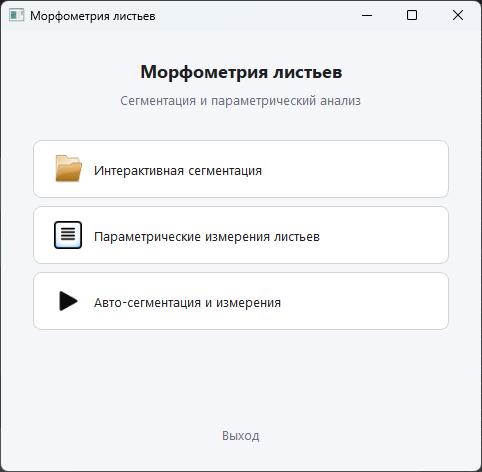
\includegraphics[width=0.5\linewidth]{figures/main_menu.png}
    \caption{Главное меню приложения}
    \label{fig:main_menu}
\end{figure}

Оба пакетных режима реализованы поверх общего конвейера обработки с подключаемыми
источниками фрагментов (см.\ раздел~\ref{sec:measure}).

\textbf{Конвенция имён файлов.} Все три источника артефактов~--- ручная сегментация
(раздел~\ref{sec:interactive}), автоматическая сегментация и параметрические
измерения (раздел~\ref{sec:auto_mode}) и
пользовательский ввод~--- порождают и потребляют файлы по единому шаблону:
\code{{stem}_leaf_crop_{idx:04d}.png} для фрагмента,
\code{{stem}_mask_{idx:04d}.png} для маски и \code{{crop_stem}_vis.png} для
визуализации измерений. Реализация и Qt-фильтры сосредоточены в модуле
\code{file_naming.py}, что позволяет смешивать в одной папке результаты разных
источников и переиспользовать их между режимами без отдельной конвертации.

\subsection{Интерактивная сегментация}
\label{sec:interactive}

Интерактивный режим (окно \texttt{SegmentationWindow}) реализует основной сценарий
работы биолога: эксперт самостоятельно выбирает листья на изображении, а система
строит маску по подсказке и при необходимости даёт инструменты ручной коррекции
(рис.~\ref{fig:segmentation_window}). Типовой рабочий цикл показан на
рис.~\ref{fig:activity}.

\begin{figure}[H]
    \centering
    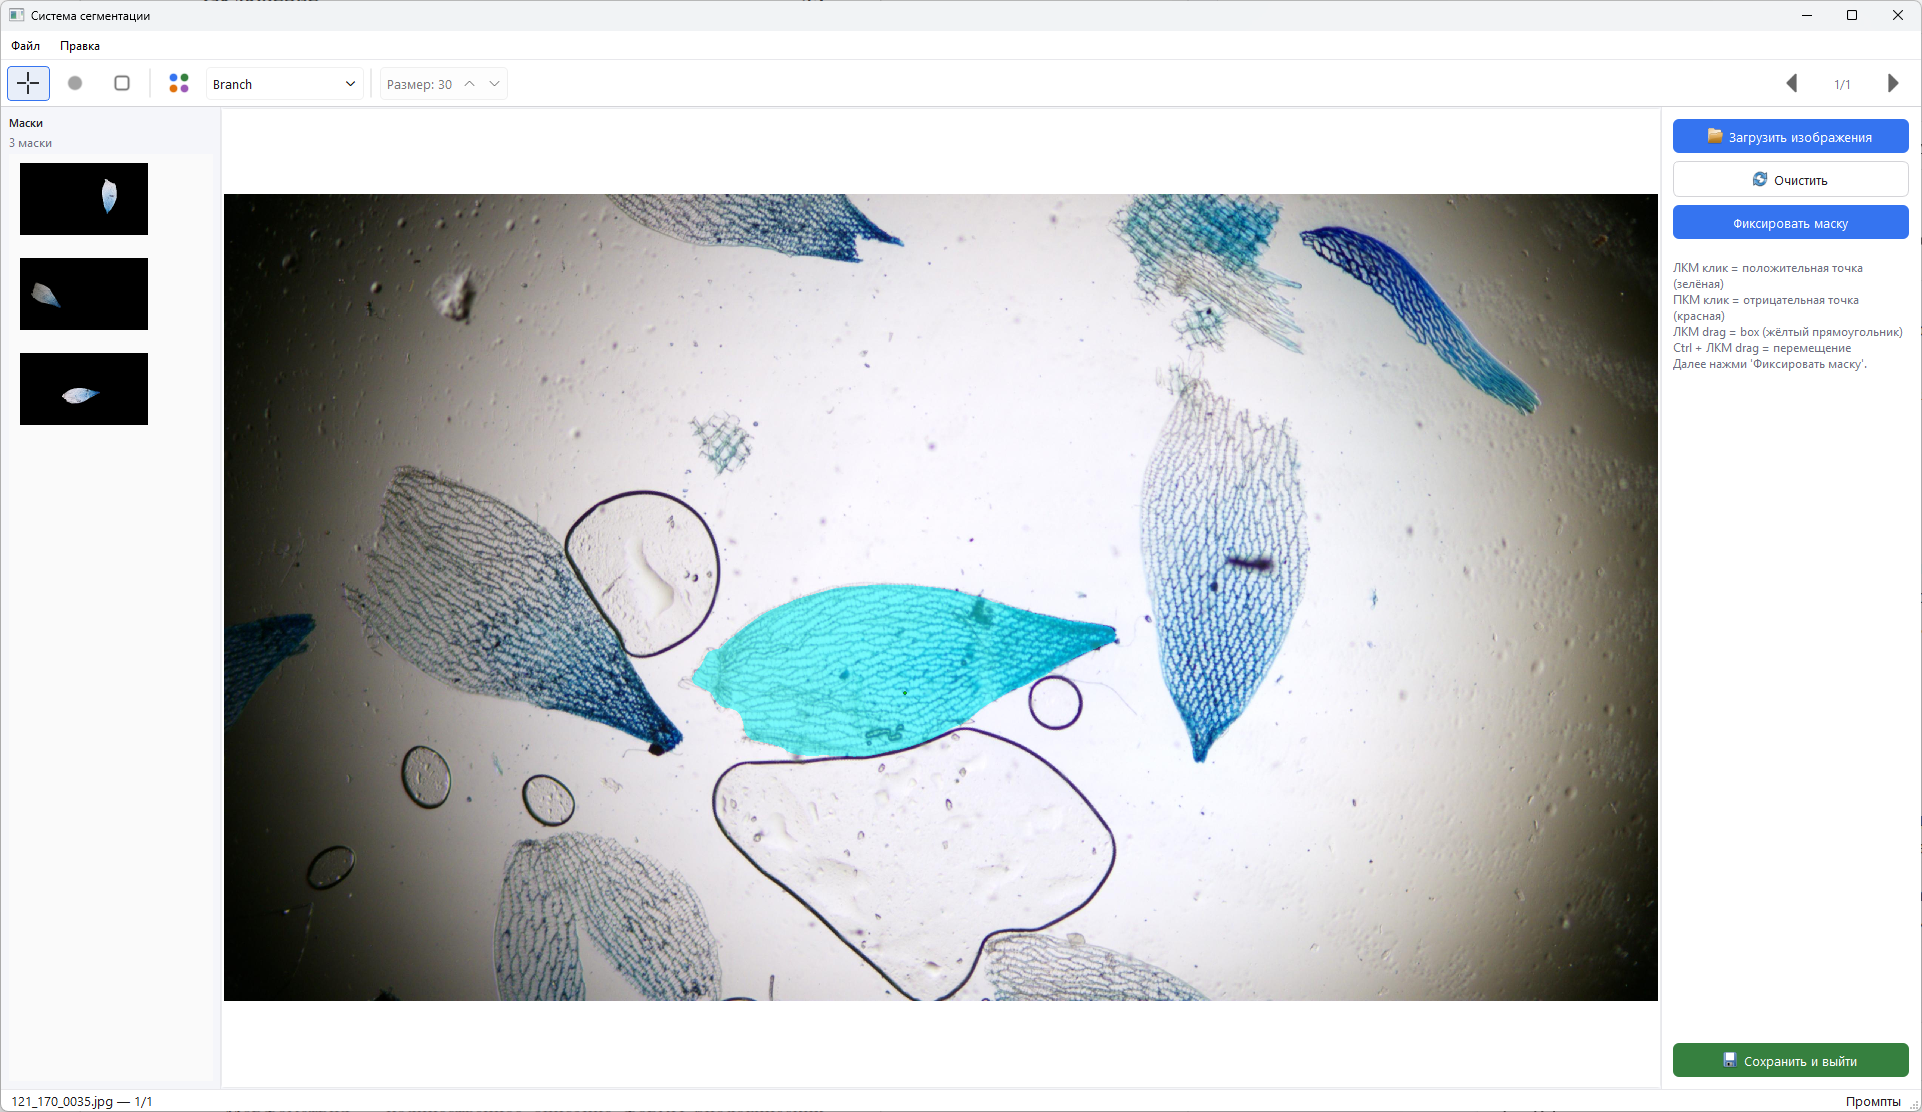
\includegraphics[width=0.95\linewidth]{figures/segmentation_canvas.png}
    \caption{Окно интерактивной сегментации}
    \label{fig:segmentation_window}
\end{figure}

\textbf{Загрузка серии и навигация.} Окно работает с серией изображений.
Загрузка набора файлов выполняется по нажатию кнопки <<Загрузить>> в боковой
панели или через пункт меню <<Файл~$\to$~Загрузить изображения>> (Ctrl+O):
выбранные снимки добавляются в очередь обработки и проходятся последовательно.
Перемещение между ними выполняется кнопками <<вперёд>> и <<назад>> в панели
инструментов; для каждого изображения сохраняется собственный буфер масок,
что позволяет накопить разметку по всей серии за один сеанс работы.

\textbf{Холст и режимы работы.} Центральный элемент интерфейса~--- \texttt{SegmentationCanvas}
на основе \texttt{QGraphicsView} с поддержкой зума к курсору и панорамирования
(\texttt{Ctrl + ЛКМ}). Холст имеет два режима. В режиме \emph{подсказок} клики
левой и правой кнопкой мыши задают позитивные и негативные опорные точки, а
перетаскивание ЛКМ~--- ограничивающий прямоугольник; после каждого изменения
автоматически вызывается \texttt{Predictor.predict}, и над изображением отображается
полупрозрачная маска. В режиме \emph{редактирования} ЛКМ работает кистью, а ПКМ~---
ластиком; диаметр кисти регулируется ползунком в панели инструментов в диапазоне $1\ldots200$~пикселей.
Маска хранится в виде ARGB-слоя (\texttt{QImage Format\_ARGB32}); переключение между
режимами не теряет промежуточный результат.

\textbf{Буфер масок.} Подтверждённые маски попадают в список \texttt{MasksBuffer}
(левая панель). Для каждой маски сохраняются два файла~--- собственно бинарная
маска и RGB-фрагмент, прошедший канонизацию (раздел~\ref{sec:pipeline}); при
выходе из окна они копируются в выбранную пользователем директорию.

\textbf{Кнопка авто-сегментации.} В панели инструментов доступна кнопка
автоматической сегментации текущего изображения~--- она запускает в фоновом
потоке тот же конвейер, что и режим автоматической сегментации и параметрических измерений
(шаги 1--4 раздела~\ref{sec:auto_mode}) для выбранного в панели типа листа. В буфер
добавляются все найденные корректные листья (рис.~\ref{fig:autosegment_result})~---
эксперту остаётся при необходимости скорректировать ошибочные маски и
доразметить пропущенные.

\begin{figure}[H]
    \centering
    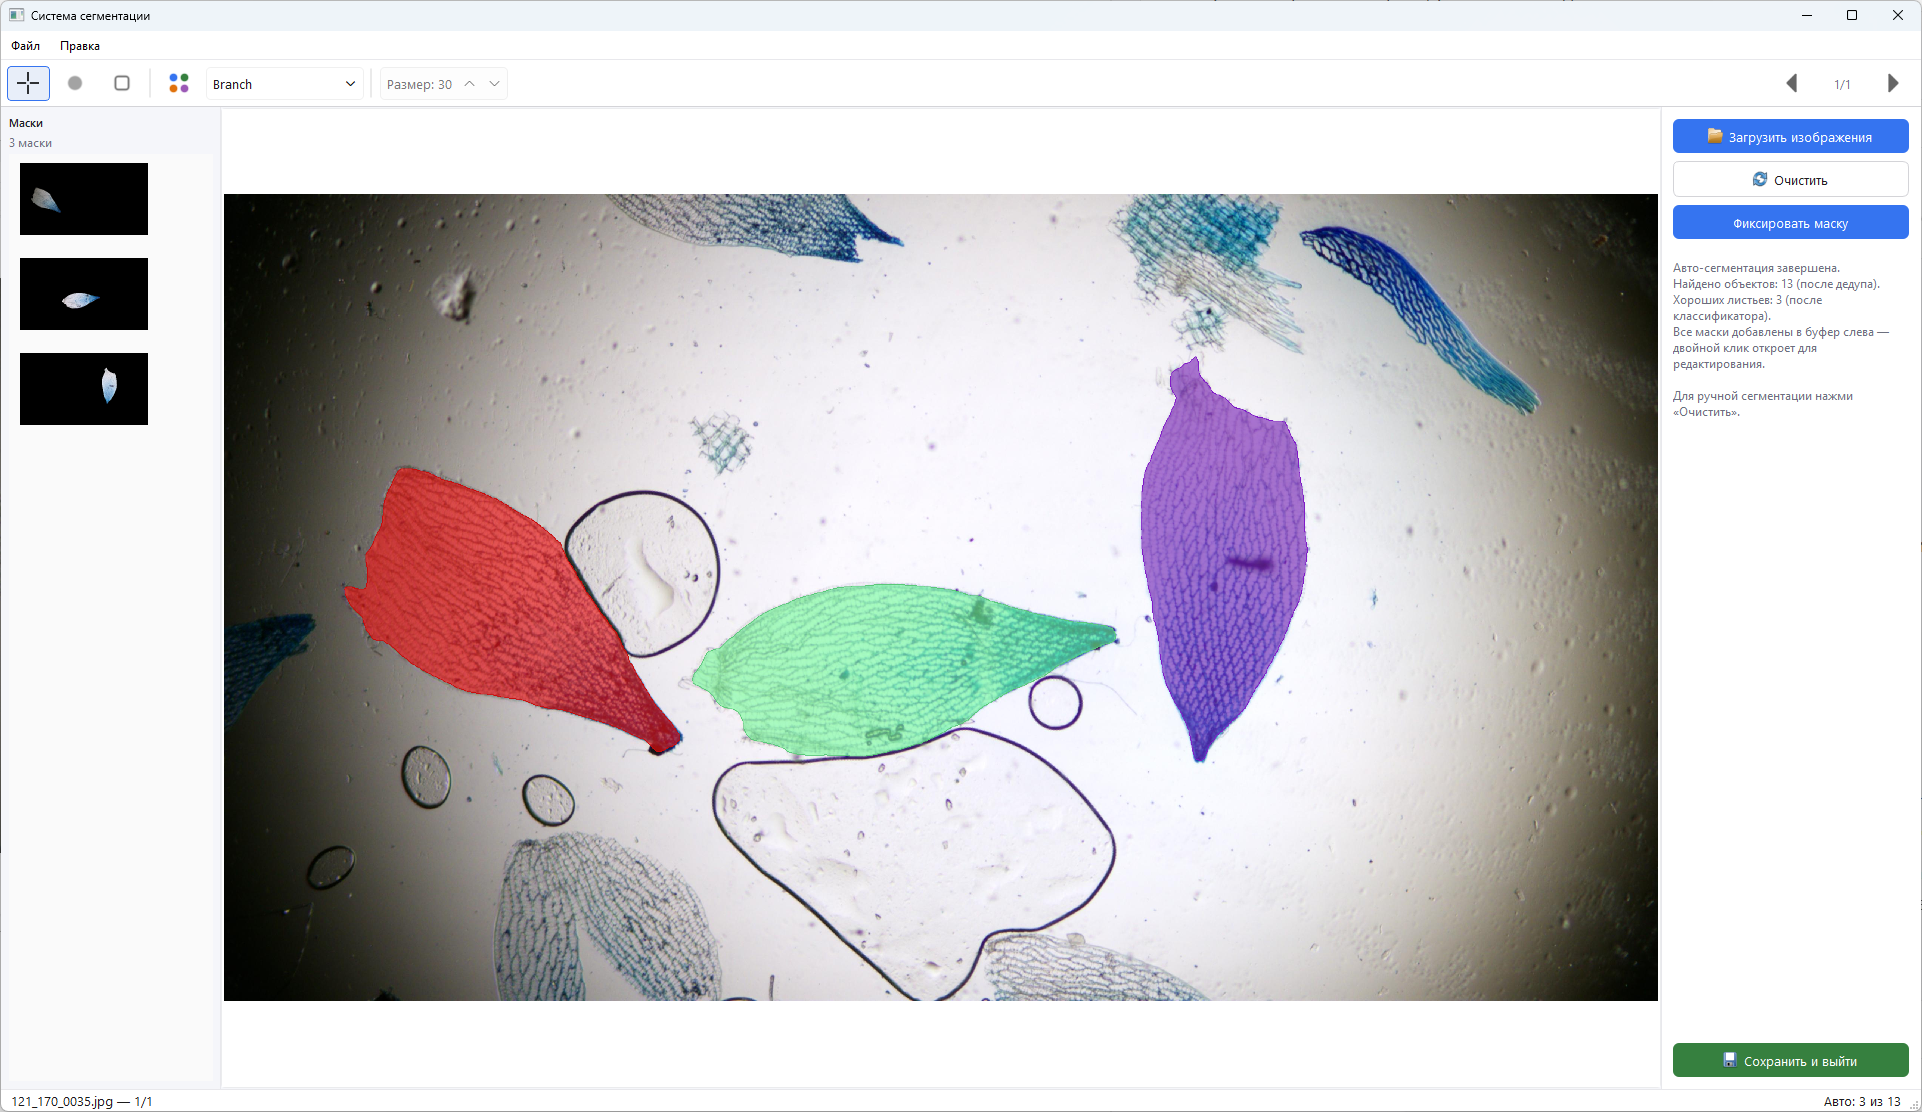
\includegraphics[width=0.95\linewidth]{figures/segmentation_canvas_autosegment_result.png}
    \caption{Результат нажатия кнопки авто-сегментации: на холсте отображены
    только листья, прошедшие классификатор отбора}
    \label{fig:autosegment_result}
\end{figure}

\begin{figure}[H]
\centering
\begin{tikzpicture}[
    font=\footnotesize,
    node distance=0.55cm,
    action/.style={rectangle, draw, rounded corners=3pt, align=center,
                   minimum width=4.8cm, minimum height=0.75cm, fill=white},
    decision/.style={diamond, draw, align=center, inner sep=1pt,
                     minimum width=1.0cm, fill=white},
    arr/.style={->, >=Stealth, thick},
    label/.style={font=\scriptsize, inner sep=1pt},
]

\node[draw, circle, fill=black, minimum size=0.28cm] (start) {};

\node[action,  below=of start]       (load)       {Загрузить папку с изображениями};
\node[action,  below=of load]        (nav)        {Перейти к следующему изображению};
\node[action,  below=of nav]         (click)      {Кликнуть на лист\\(positive point / bbox)};
\node[action,  below=of click]       (sam)        {\textit{[система]} Построить маску (MobileSAM)};
\node[decision,below=of sam]         (ok)         {Маска\\точная?};
\node[action,  below=of ok]          (save)       {\textit{[система]} Сохранить маску в буфер};
\node[decision,below=of save]        (moreleaves) {Ещё листья\\на изображении?};
\node[decision,below=of moreleaves]  (moreimages) {Ещё\\изображения?};
\node[action,  below=of moreimages]  (savebuf)    {Сохранить буфер масок\\и канонизированных фрагментов\\в выбранную папку};

\node[draw, circle, fill=black, minimum size=0.28cm,
      below=of savebuf] (end) {};
\node[draw, circle, minimum size=0.38cm] at (end) {};

\node[action, right=1.8cm of ok] (edit) {Исправить маску\\(кисть / ластик)};

\draw[arr] (start) -- (load);
\draw[arr] (load)  -- (nav);
\draw[arr] (nav)   -- (click);
\draw[arr] (click) -- (sam);
\draw[arr] (sam)   -- (ok);

\draw[arr] (ok)       -- node[label, left]{да} (save);
\draw[arr] (ok.east)  -- node[label, above]{нет} (edit.west);
\draw[arr] (edit.south) |- (save.east);

\draw[arr] (save) -- (moreleaves);

\draw[arr] (moreleaves) -- node[label, left]{нет} (moreimages);
\draw[arr] (moreleaves.west) -- ++(-2.0,0) node[label, above left]{да}
           |- (click.west);

\draw[arr] (moreimages) -- node[label, left]{нет} (savebuf);
\draw[arr] (moreimages.west) -- ++(-3.0,0) node[label, above left]{да}
           |- (nav.west);

\draw[arr] (savebuf) -- (end);

\end{tikzpicture}
\caption{Диаграмма активностей: рабочий цикл пользователя в интерактивном режиме}
\label{fig:activity}
\end{figure}

\subsection{Канонизация листа}
\label{sec:pipeline}

Маска, полученная сегментирующей моделью или ручной коррекцией, ориентирована
произвольно и может содержать мелкие артефакты~--- отдельные пиксели и
внутренние дыры. Перед измерениями и классификацией её приводят к стандартному
\emph{каноническому} виду: главная ось листа расположена вертикально, апекс
направлен вверх, фон обнулён, а контур очищен от артефактов
(рис.~\ref{fig:pipeline_stages}).

В этом виде фрагмент используется во всех последующих этапах обработки: на
канонических фрагментах работает алгоритм параметрических измерений
(раздел~\ref{sec:measure}), на них же обучается и применяется классификатор
отбора (глава~\ref{sec:classifier_chapter}); кроме того, канонический фрагмент
встраивается в визуализации и таблицы экспорта.

\begin{figure}[H]
    \centering
    \begin{tabular}{c@{\hspace{0.2cm}}c@{\hspace{0.2cm}}c@{\hspace{0.2cm}}c@{\hspace{0.2cm}}c}
        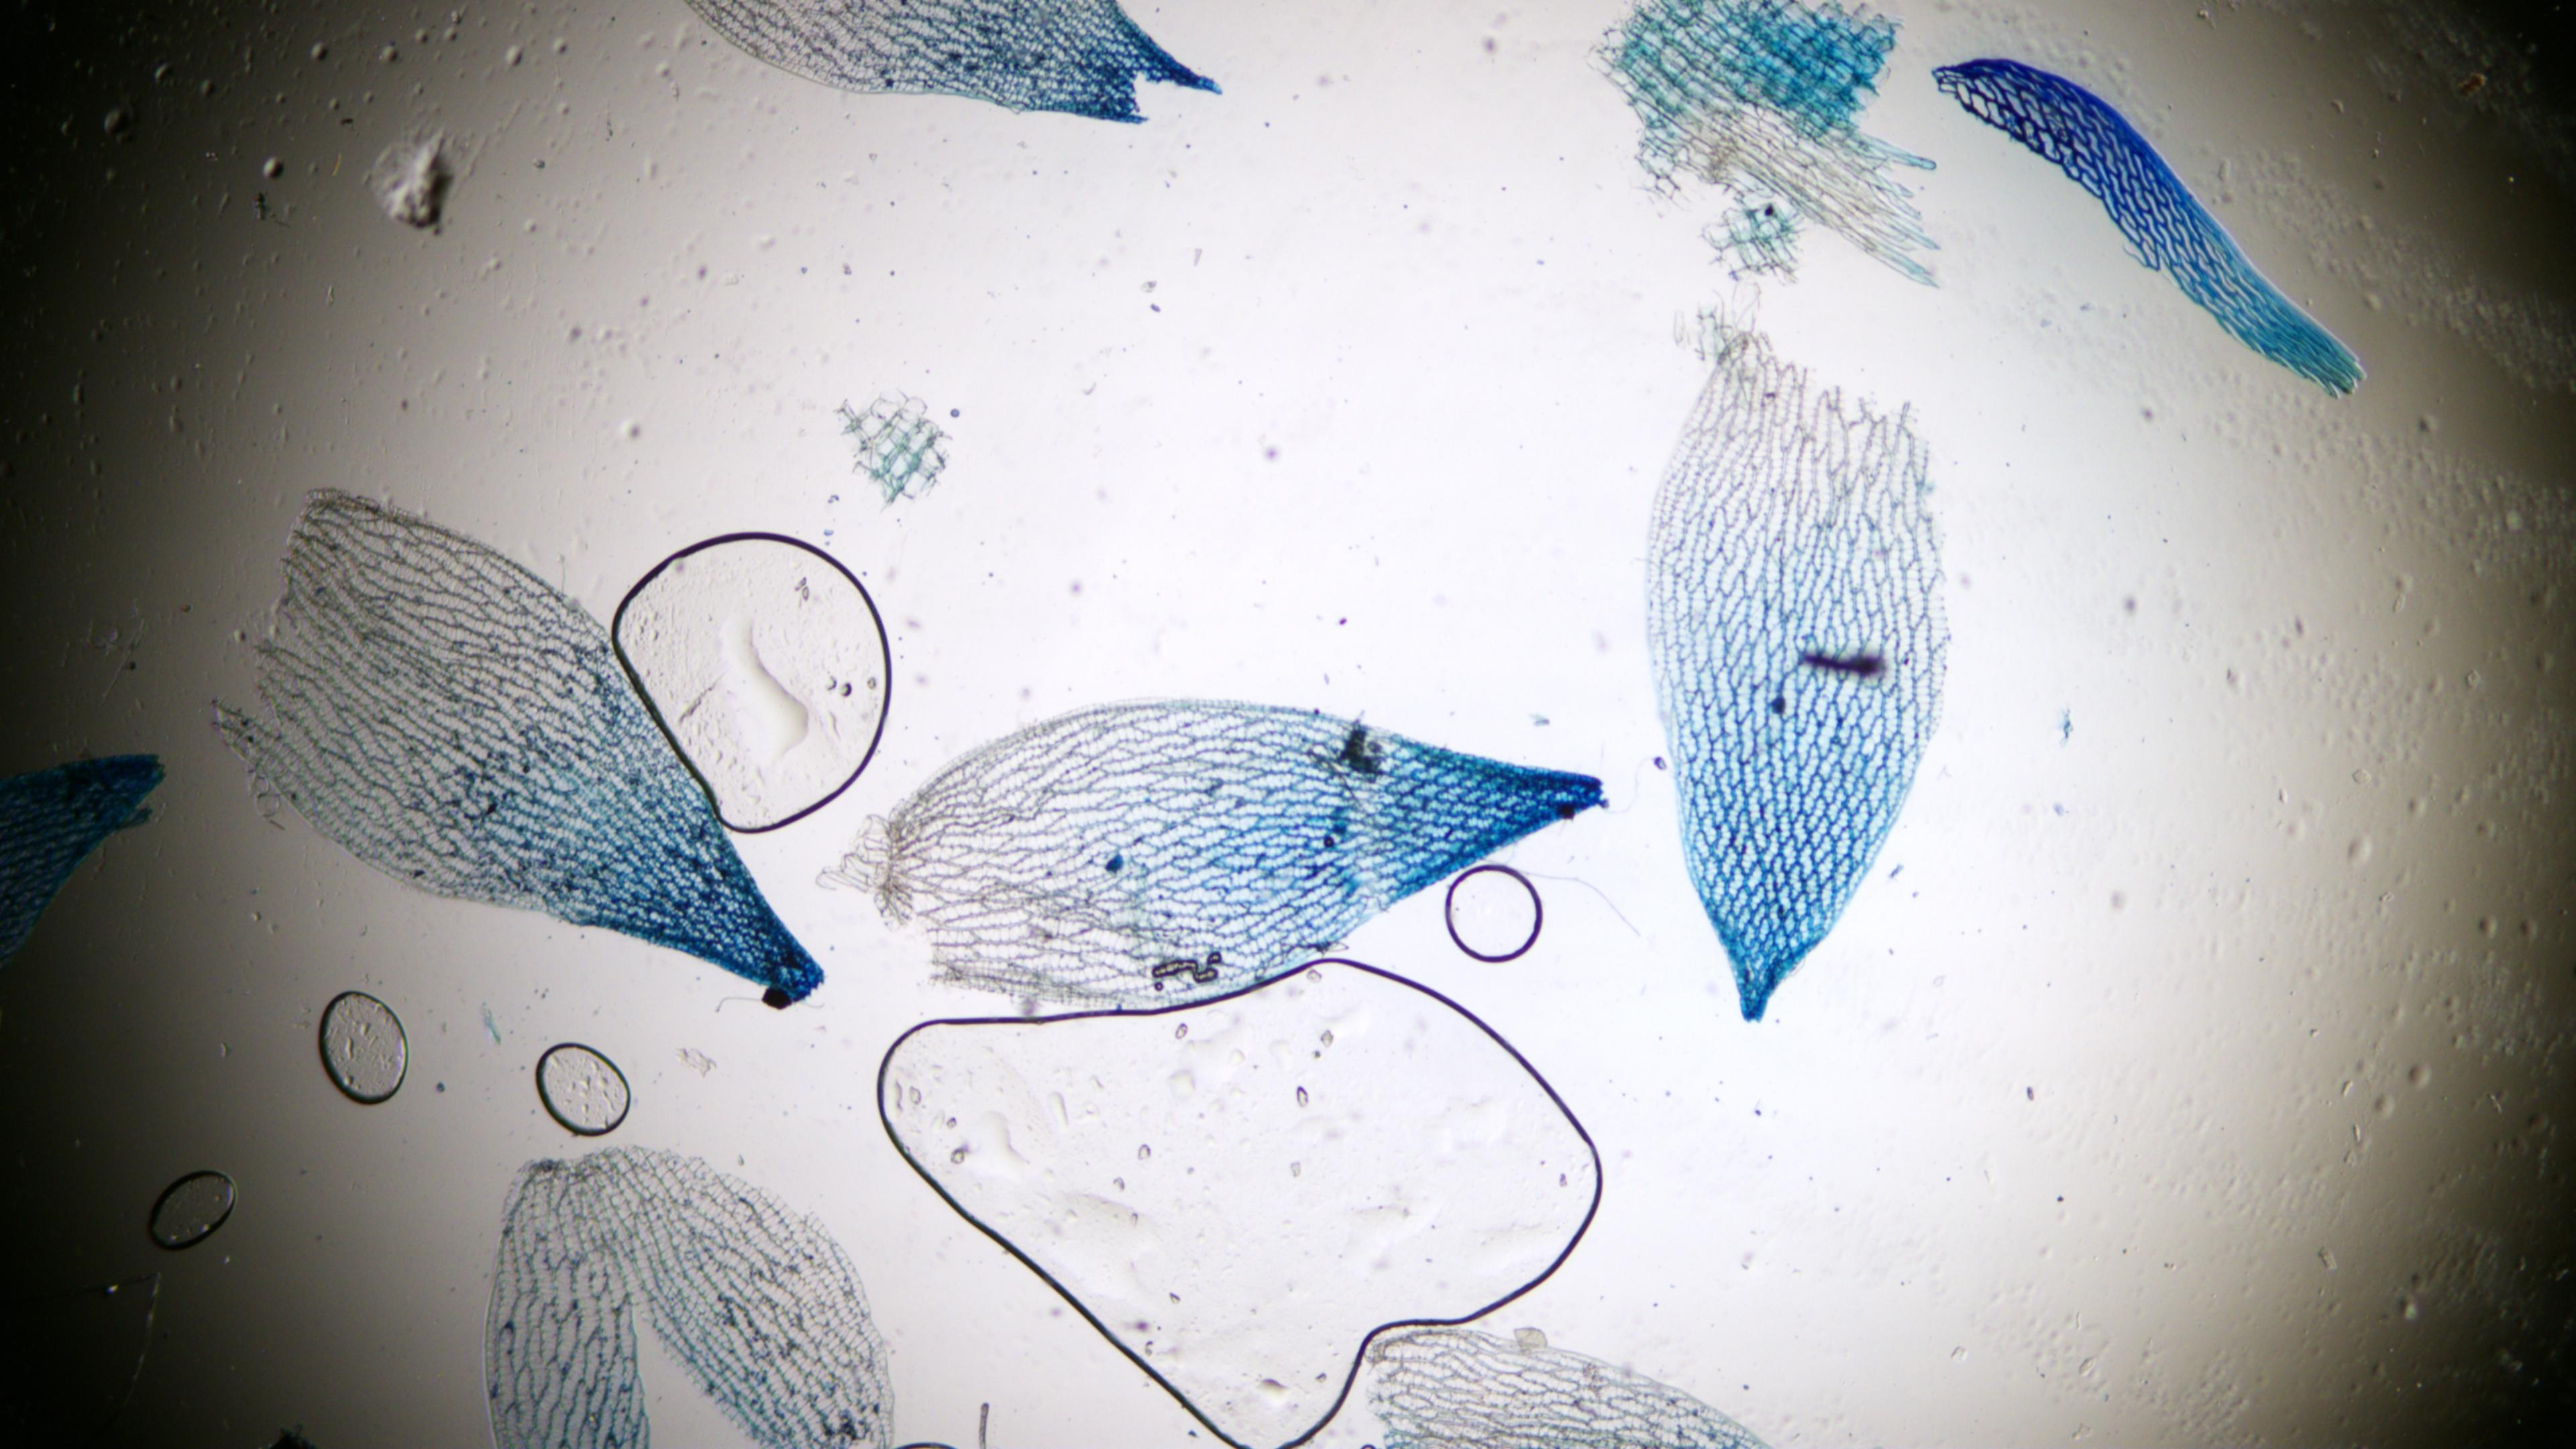
\includegraphics[height=2.8cm]{figures/121_170_0035.jpg} &
        \raisebox{1.2cm}{\Large$\to$} &
        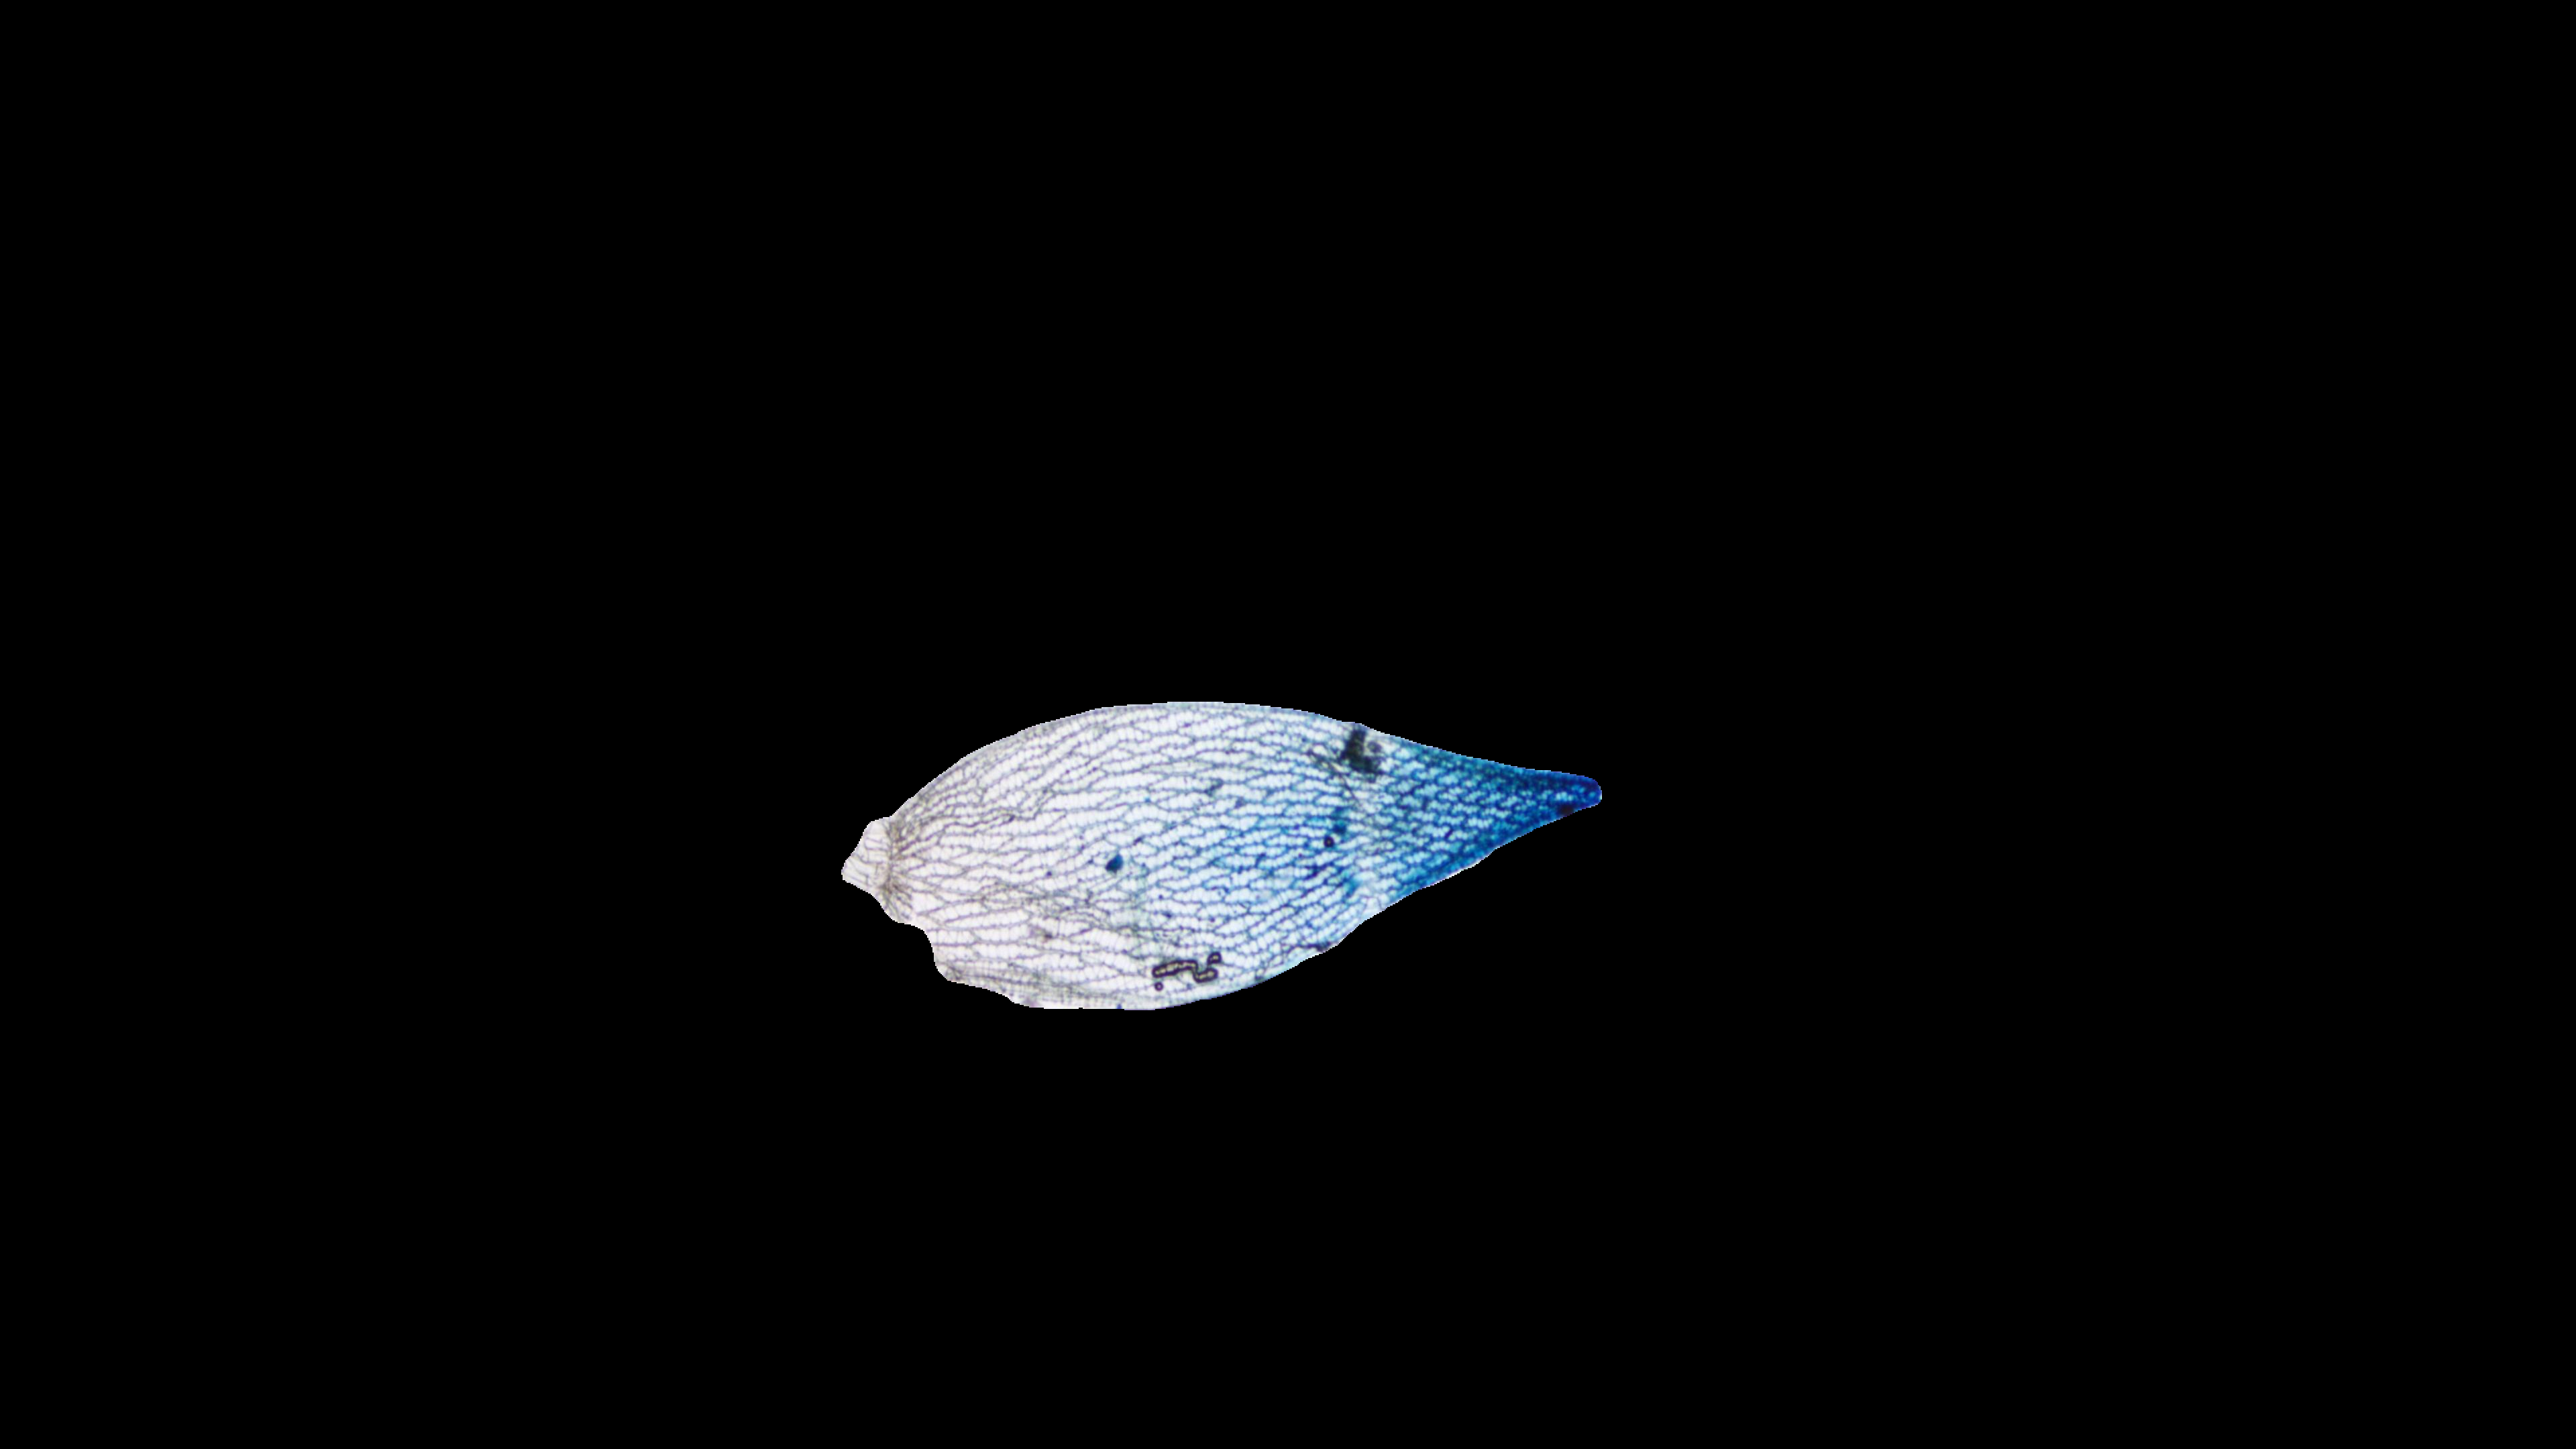
\includegraphics[height=2.8cm]{figures/121_170_0035_mask_0002.png} &
        \raisebox{1.2cm}{\Large$\to$} &
        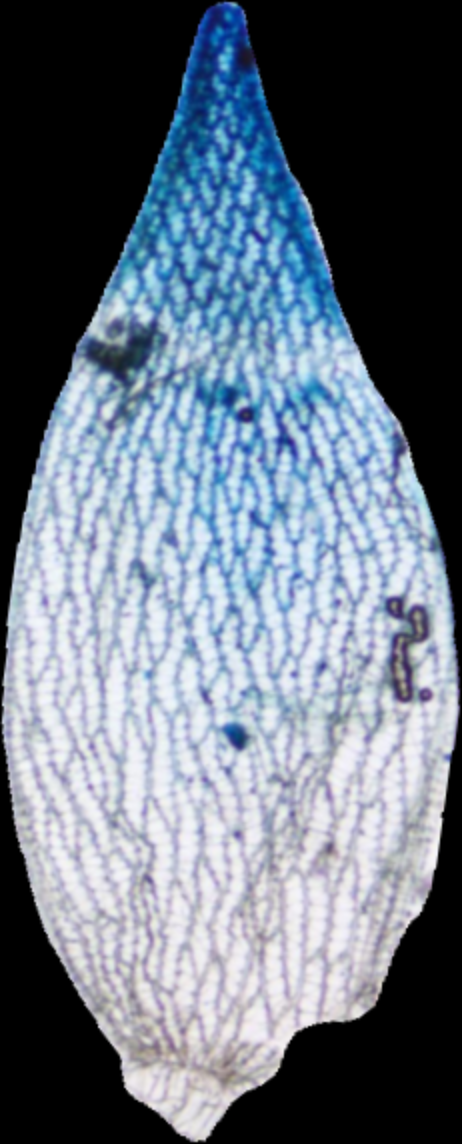
\includegraphics[height=2.8cm]{figures/121_170_0035_leaf_crop_0002.png} \\[2pt]
        {\footnotesize (а) исходное} & &
        {\footnotesize (б) маска} & &
        {\footnotesize (в) фрагмент} \\
    \end{tabular}
    \caption{Преобразование листа в конвейере: исходное изображение $\to$ очищенная
    маска $\to$ канонизированный фрагмент}
    \label{fig:pipeline_stages}
\end{figure}

Канонизация реализована в модуле \texttt{leaf\_pipeline.py} и состоит из двух шагов.

\textbf{Шаг 1: очистка маски (\texttt{preprocess\_mask}).} Реализация: поиск
всех внешних контуров через \texttt{cv2.findContours}, выбор контура максимальной
площади и заполнение получившейся области через \texttt{cv2.drawContours} с
флагом \texttt{FILLED}. На выходе~--- маска \texttt{uint8} (0 либо 255),
содержащая ровно одну связную компоненту без дыр.

\textbf{Шаг 2: канонизация ориентации (\texttt{pca\_crop}).} Ориентация листа
определяется методом главных компонент (Principal Component Analysis,
PCA)~\cite{Jolliffe2002}: по координатам активных пикселей маски строится
матрица ковариации $2 \times 2$, её собственные векторы вычисляются через
\texttt{np.linalg.eigh}. Собственный вектор с наибольшим собственным значением
указывает направление наибольшего разброса пикселей листа~--- то есть его
удлинённую (главную) ось. Изображение с обнулённым фоном поворачивается
аффинным преобразованием так, чтобы главная ось совпадала с вертикалью. После
поворота определяется направление апекса: если в верхней половине bbox больше
активных пикселей, чем в нижней, изображение переворачивается по вертикали~---
так апекс всегда оказывается сверху. Финальный шаг~--- обрезка по плотному
bounding box активных пикселей; выходом является RGB-фрагмент, в котором лист
занимает почти всю площадь и ориентирован вертикально.

\subsection{Параметрические измерения листа}
\label{sec:measure}

\subsubsection*{Алгоритм измерений}

Модуль \texttt{leaf\_measure.py} принимает на вход RGB-фрагмент в каноническом
виде (раздел~\ref{sec:pipeline}): главная ось вертикальна, апекс сверху,
фон обнулён. Это позволяет отказаться от повторного построения контура и
анализа главных компонент: все измерения сводятся к работе с маской активных
пикселей в системе координат самого фрагмента (рис.~\ref{fig:measurement}).

\begin{figure}[H]
    \centering
    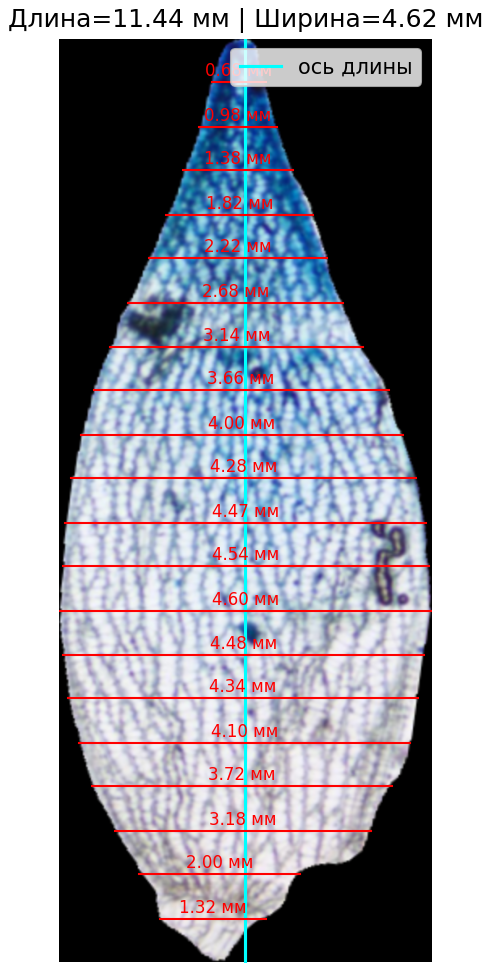
\includegraphics[width=0.22\linewidth]{figures/metrics_visualization.png}
    \caption{Визуализация измерений одного листа: длина и семь поперечных сечений}
    \label{fig:measurement}
\end{figure}

\textbf{Длина и максимальная ширина.} Длина листа определяется как высота
прямоугольника, ограничивающего активные пиксели фрагмента: $L = (y_{\max} - y_{\min} + 1) \cdot s$,
где $s$~--- масштабный коэффициент (мм/пиксель), равный единице, если пользователь
работает в пикселях. Максимальная ширина~--- ширина того же прямоугольника:
$W = (x_{\max} - x_{\min} + 1) \cdot s$.

\textbf{Поперечные сечения.} Для каждой доли $f \in (0, 1)$ берётся строка
$y = y_{\min} + \mathrm{round}\bigl(f \cdot (y_{\max} - y_{\min})\bigr)$. В этой
строке находятся крайний левый и крайний правый ненулевые пиксели $x_l$ и
$x_r$; ширина в сечении равна $w_f = (x_r - x_l + 1) \cdot s$. По умолчанию
используются семь сечений с долями
$0{,}125;\; 0{,}25;\; 0{,}375;\; 0{,}5;\; 0{,}625;\; 0{,}75;\; 0{,}875$, что
соответствует равномерному разбиению длины листа на восемь интервалов.

\textbf{Результат.} Метод возвращает структуру \texttt{LeafMetrics} с полями
\texttt{length}, \texttt{width} и словарём \texttt{widths: dict[float, SectionWidth]}~---
для каждой доли хранятся сама ширина и координаты крайних точек.

\subsubsection*{Режим замеров по готовым фрагментам}

Пакетный режим запускается из главного меню и используется, когда канонические
фрагменты уже подготовлены ранее: сохранены интерактивным режимом сегментации
(раздел~\ref{sec:interactive}), получены автоматическим режимом
(раздел~\ref{sec:auto_mode}) или предоставлены пользователем напрямую. Параметры
запуска задаются в диалоге настроек (рис.~\ref{fig:settings_dialog}): набор
файлов, выходная директория, число поперечных сечений, масштабный коэффициент,
формат экспорта (по умолчанию~--- CSV).

\begin{figure}[H]
    \centering
    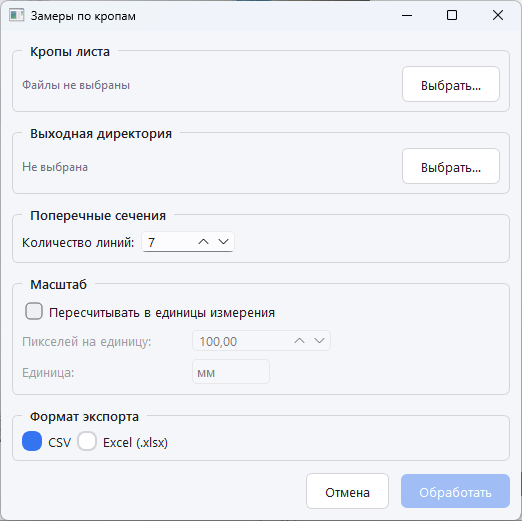
\includegraphics[width=0.6\linewidth]{figures/measure_metrics_settings_menu.png}
    \caption{Диалог настроек пакетной обработки}
    \label{fig:settings_dialog}
\end{figure}

Каждый выбранный файл читается с диска по принятой конвенции имён
(раздел~\ref{sec:architecture}) и подаётся на алгоритм измерений; результаты
по всей серии накапливаются и в конце экспортируются в таблицу. По завершении
пользователь получает диалог с числом обработанных файлов, числом ошибок и
путём к итоговой таблице. Ошибки на отдельных файлах не прерывают пакет~---
они накапливаются в результате и отображаются по окончании.

Помимо таблицы, для каждого обработанного фрагмента сохраняется изображение
\texttt{*\_vis.png} с нанесённой осью длины и поперечными сечениями
(см.\ рис.~\ref{fig:measurement}). В режиме экспорта в XLSX миниатюра этой
визуализации встраивается в ячейку таблицы, что позволяет биологу визуально
оценить корректность измерений непосредственно в Excel, не открывая файлы по
отдельности.

\subsection{Автоматическая сегментация и параметрические измерения}
\label{sec:auto_mode}

В этом режиме система обрабатывает серию изображений без участия пользователя. Конвейер обработки одного снимка состоит из пяти шагов;
на выходе всей серии~--- сводная таблица морфометрических измерений. Первые
три шага реализованы единой функцией \texttt{auto\_segment} (модуль
\texttt{leaf\_pipeline.py}).

\textbf{Шаг 1: генерация кандидатов.} Запускается \texttt{SamAutomaticMaskGenerator}.
Маски, площадь которых меньше $0{,}1\,\%$ или больше $70\,\%$ кадра,
отфильтровываются.

\textbf{Шаг 2: дедупликация.} AMG генерирует десятки масок-кандидатов; среди
них часто встречаются дубликаты~--- несколько масок одного и того же листа
разных размеров. Маски сортируются по убыванию площади и попарно отбрасываются
по порогу IoU $> 0{,}9$.

\textbf{Шаг 3: канонизация.} К каждой выжившей маске применяется конвейер
канонизации листа (раздел~\ref{sec:pipeline}). Результатом \texttt{auto\_segment}
является список пар (очищенная маска, канонический RGB-фрагмент).

\textbf{Шаг 4: фильтрация классификатором отбора.} Каждый канонический
фрагмент маркируется обученным классификатором (глава~\ref{sec:classifier_chapter})
одним из трёх классов; в итоговую таблицу попадают только фрагменты класса
\texttt{good\_leaf}.

\textbf{Шаг 5: расчёт параметров и экспорт.} К каждому отобранному фрагменту
применяется тот же алгоритм параметрических измерений, что и в режиме замеров
по готовым фрагментам (раздел~\ref{sec:measure}); результаты по всей серии
накапливаются и экспортируются в сводную таблицу. Помимо таблицы, для каждого
фрагмента сохраняются маска и канонический RGB-фрагмент в подпапках
\texttt{masks/} и \texttt{crops/} выходной директории.

Режим открывается из главного меню; диалог настроек тот же, что у режима
замеров, с одним дополнительным полем~--- выпадающим списком выбора типа листа,
по которому подгружается соответствующая модель отбора. По умолчанию формат
экспорта~--- XLSX со встроенными миниатюрами визуализаций измерений в столбце
\texttt{crop}.

\subsection{Оптимизация производительности автоматической сегментации}
\label{sec:auto_perf}

Прямолинейная реализация на ноутбуке без GPU обрабатывала один кадр $3840 \times 2160$ за
$\approx 17{,}7$~с от нажатия кнопки до отображения масок, что почти вдвое
превышает предусмотренный требованиями (раздел~\ref{sec:requirements}) бюджет в
10~с на изображение. Последовательное применение семи оптимизаций снизило это
время до $\approx 1{,}0$~с (рис.~\ref{fig:auto_perf}). Замеры выполнены на 4K-кадре с
13 масками.

\begin{figure}[H]
\centering
\begin{tikzpicture}
\definecolor{cSam}{HTML}{4E79A7}
\definecolor{cDedup}{HTML}{F28E2B}
\definecolor{cScale}{HTML}{59A14F}
\definecolor{cSave}{HTML}{E15759}
\definecolor{cClass}{HTML}{76B7B2}
\begin{axis}[
    xbar stacked,
    width=\linewidth,
    height=12.5cm,
    bar width=0.35cm,
    xmin=0, xmax=19,
    xlabel={Время, с},
    xlabel style={font=\footnotesize},
    xticklabel style={font=\footnotesize},
    xticklabel={\pgfmathprintnumber[/pgf/number format/use comma]{\tick}},
    symbolic y coords={v7,v6,v5,v4,v3,v2,v1,v0},
    ytick=\empty,
    legend style={at={(0.5,-0.12)}, anchor=north, legend columns=5,
                  font=\footnotesize, draw=none,
                  /tikz/every even column/.append style={column sep=0.5cm}},
    legend cell align=left,
    xmajorgrids,
    major grid style={dotted, gray!50},
    axis line style={draw=gray!60},
    tick style={draw=gray!60},
    enlarge y limits=0.08,
]
\addplot+[draw=none, fill=cSam]   coordinates {(6.10,v0) (0.30,v1) (0.30,v2) (0.30,v3) (0.30,v4) (0.30,v5) (0.30,v6) (0.30,v7)};
\addplot+[draw=none, fill=cDedup] coordinates {(8.54,v0) (4.99,v1) (1.17,v2) (1.16,v3) (1.17,v4) (0.93,v5) (0.28,v6) (0.28,v7)};
\addplot+[draw=none, fill=cScale] coordinates {(0.00,v0) (0.00,v1) (2.89,v2) (0.69,v3) (0.10,v4) (0.10,v5) (0.10,v6) (0.10,v7)};
\addplot+[draw=none, fill=cClass] coordinates {(0.15,v0) (0.15,v1) (0.15,v2) (0.15,v3) (0.15,v4) (0.15,v5) (0.15,v6) (0.15,v7)};
\addplot+[draw=none, fill=cSave]  coordinates {(2.89,v0) (2.86,v1) (2.84,v2) (2.89,v3) (2.90,v4) (2.90,v5) (1.62,v6) (0.17,v7)};
\legend{SAM, дедупликация, масштабирование, классификатор, сохранение}
% Подписи шагов над барами
\node[anchor=south west, font=\footnotesize, yshift=4pt] at (axis cs:0,v0) {0. Исходная реализация};
\node[anchor=south west, font=\footnotesize, yshift=4pt] at (axis cs:0,v1) {1. Понижение разрешения для сегментации};
\node[anchor=south west, font=\footnotesize, yshift=4pt] at (axis cs:0,v2) {2. Понижение разрешения для дедупликации};
\node[anchor=south west, font=\footnotesize, yshift=4pt] at (axis cs:0,v3) {3. Сокращение копирования при масштабировании};
\node[anchor=south west, font=\footnotesize, yshift=4pt] at (axis cs:0,v4) {4. Однократная канонизация};
\node[anchor=south west, font=\footnotesize, yshift=4pt] at (axis cs:0,v5) {5. Локальный IoU при дедупликации};
\node[anchor=south west, font=\footnotesize, yshift=4pt] at (axis cs:0,v6) {6. Сокращение копирования при дедупликации};
\node[anchor=south west, font=\footnotesize, yshift=4pt] at (axis cs:0,v7) {7. Асинхронное сохранение};
% Итоги справа от баров
\node[anchor=west, font=\scriptsize\bfseries] at (axis cs:17.68,v0) {17{,}7};
\node[anchor=west, font=\scriptsize\bfseries] at (axis cs:8.30,v1)  {8{,}3};
\node[anchor=west, font=\scriptsize\bfseries] at (axis cs:7.35,v2)  {7{,}4};
\node[anchor=west, font=\scriptsize\bfseries] at (axis cs:5.19,v3)  {5{,}2};
\node[anchor=west, font=\scriptsize\bfseries] at (axis cs:4.62,v4)  {4{,}6};
\node[anchor=west, font=\scriptsize\bfseries] at (axis cs:4.38,v5)  {4{,}4};
\node[anchor=west, font=\scriptsize\bfseries] at (axis cs:2.45,v6)  {2{,}5};
\node[anchor=west, font=\scriptsize\bfseries] at (axis cs:1.00,v7)  {1{,}0};
\end{axis}
\end{tikzpicture}
\caption{Время одного 4K-кадра в конвейере автоматической сегментации по шагам
оптимизации}
\label{fig:auto_perf}
\end{figure}

Семь шагов из диаграммы группируются в пять приёмов.

\textbf{Понижение входного разрешения} (шаги~1--2). Кодировщик SAM
принудительно приводит вход к квадрату $1024 \times 1024$, поэтому стоимость
самого инференса от исходного разрешения не зависит, но пост-обработка масок
(немаксимальное подавление, фильтрация по \texttt{stability\_score})
масштабируется как $O(W \cdot H \cdot N)$. Подача на вход AMG вдвое
уменьшенной копии кадра ускорила сегментацию приблизительно в 13 раз.
Аналогично, дедупликация и канонизация выполняются на той же уменьшенной
копии~--- до финального масштабирования выживших масок к исходному
разрешению,~--- что сократило время дедупликации приблизительно в 4 раза.

\textbf{Сокращение копирования кадра} (шаги~3, 6). В двух циклах~--- финальном
масштабировании и канонизации внутри дедупликации~--- для каждой маски
выполнялась полная копия кадра ($\approx 25$~МБ для исходного разрешения и
$\approx 6$~МБ для уменьшенной копии), после чего пиксели вне маски обнулялись.
Замена на копирование только области, ограниченной маской, устранила сотни
мегабайт лишних данных и существенно ускорила аффинные преобразования.

\textbf{Локальный IoU при дедупликации} (шаг~5). Изначально попарный IoU между
двумя масками считался в лоб: \texttt{logical\_and} и \texttt{logical\_or} по
всем $H \times W$ пикселям обеих масок~--- два полных прохода на каждую пару
при $\sim 17$ масках-кандидатах. Замена устроена в два шага. Во-первых, перед
попарным сравнением проверяется пересечение ограничивающих прямоугольников
масок: если прямоугольники не пересекаются, маски заведомо не пересекаются и
$\text{IoU} = 0$~--- пара отсеивается без единого пиксельного сравнения.
Во-вторых, для пересекающихся прямоугольников \texttt{logical\_and} вычисляется
только в области их пересечения, а объединение~--- по формуле
$|A \cup B| = |A| + |B| - |A \cap B|$ из заранее посчитанных площадей и только
что найденного пересечения, без второго полного прохода.

\textbf{Однократная канонизация} (шаг~4). Дедупликация уже выполняла
канонизацию каждого выжившего листа на уменьшенной копии кадра, а финальный
цикл масштабирования игнорировал этот результат и канонизировал тот же лист
повторно на полном разрешении. Замена на билинейное масштабирование уже
канонизированного фрагмента к нужному размеру избавила от двойной работы.
Возникающее размытие в~2--3 пикселя некритично.

\textbf{Асинхронное сохранение} (шаг~7). Запись масок на диск синхронно с
интерфейсом давала $\approx 2{,}9$~с зависания. Запись вынесена в фоновый пул
потоков; для отрисовки миниатюр $128 \times 128$ один раз на изображение
строится уменьшенная копия исходника ($\approx 250$~КБ вместо 25~МБ), из которой
и берутся все иконки. Интерфейс больше не блокируется на сохранение, а
синхронизация с фоновыми записями выполняется только там, где она действительно
нужна: при сохранении результатов и выходе из окна ждём завершения всех записей
перед копированием файлов в выходную папку, а при редактировании или удалении
уже сохранённой маски ждём её конкретной записи, чтобы перечитать файл с диска.

\textbf{Итог.} Время обработки одного 4K-кадра сократилось с 17{,}7 до
1{,}0~с~--- примерно в восемнадцать раз. Кнопка авто-сегментации в окне
интерактивной разметки (раздел~\ref{sec:interactive}) теперь отрабатывает за
секунду: задержка приемлема для интерактивного использования.

\subsection{Тестирование}
\label{sec:testing}

Все тесты исполняются автоматически
при каждом пуше через GitHub~Actions; внешние тяжёлые зависимости
(MobileSAM, XGBoost-модели классификатора) подменяются заглушками, что
позволяет CI работать без GPU и без модельных весов.

\textbf{Модульные тесты} ($\approx 160$ случаев) покрывают чистые функции
ядра: конвенцию имён артефактов, чтение изображений и русское склонение,
препроцессинг маски и PCA-канонизацию, API измерителя, экспорт CSV/XLSX,
конвейер обработки и адаптеры классификатора. Граничные случаи
(пустая маска, одна компонента из нескольких, дыры в маске, отсутствие
пикселей листа в выбранной строке) выделены в отдельные параметризованные
сценарии.

\textbf{Контроль точности измерений} (категория~1) выполняется на
контрольной выборке из 9 снимков, для которых эксперт-биолог вручную
замерил длину листа и семь поперечных ширин в пикселях. Тест загружает
изображение и заранее подготовленную маску, прогоняет
\texttt{transform\_leaf} и \texttt{measure\_leaf}, сверяет результат
с эталоном по критерию $\max(\delta_{\text{отн}}, \delta_{\text{абс}})$:
для длины~--- $3\,\%$, для сечений~--- $5\,\%$.

\textbf{Регрессия автосегментации} (категория~2) использует подход
\emph{golden master}: для каждого снимка контрольной выборки сохранены
площадь и центр масс всех масок, выданных текущей версией
\texttt{auto\_segment}. При повторных прогонах допускается отклонение
площади до $2\,\%$ и центра~--- до $5$~пикселей. Тест ловит регрессии
при оптимизациях конвейера, но не претендует на абсолютную меру
качества сегментации, поскольку эталон сгенерирован самим алгоритмом.

\subsection{Сборка и публикация}
\label{sec:packaging}

Целевая аудитория~--- сотрудники биологической лаборатории, для которых
установка Python и его зависимостей не является штатной операцией. Доставка
реализована в виде автономной сборки под Windows~64 на базе PyInstaller~6.11.1
в режиме \texttt{-{}-onedir}, включающей интерпретатор Python, все библиотеки и
веса моделей. Сборка использует только CPU и не требует ни предустановленного
Python, ни системных зависимостей, ни GPU.

Итоговая сборка занимает $\approx 920$~МБ и распространяется в виде
RAR-архива ($\approx 327$~МБ); готовые сборки опубликованы в разделе
\href{https://github.com/pavelrubanov/segmentation_system/releases}{Releases}
репозитория проекта. Запуск~--- двойным кликом по \texttt{sphagnum.exe};
стандартные потоки перенаправляются в файлы \texttt{stdout.log} и
\texttt{stderr.log} в её директории.

